\documentclass[11pt]{article}
\usepackage[margin=1in]{geometry}
\usepackage{booktabs}
\usepackage{graphicx}
\usepackage{hyperref}
\usepackage{enumitem}
\usepackage{microtype}

\title{An Explainable Diabetes-Risk Digital Twin:\\Four Stage-Wise Experiments on BRFSS Survey Data}
\author{Anonymous}
\date{}

\begin{document}
\maketitle

\begin{abstract}
Machine-learning models can estimate diabetes-related survey labels, but a useful research prototype must also expose model evidence, support transparent scenario analysis, and communicate limitations. We evaluate an explainable diabetes-risk Digital Twin through four linked experiments: three-class prediction, global and patient-level explanation, manual what-if simulation with a 3D representation, and knowledge-graph-based evidence integration with constrained local-language-model guidance. A 400-tree class-weighted Random Forest trained on 253,680 CDC BRFSS 2015 records achieved 81.96\% accuracy, 45.06\% balanced accuracy, 44.37\% macro-F1, and 0.758 macro one-vs-rest ROC-AUC; however, Medium/prediabetes recall was only 0.11\%. In one held-out High/diabetes case, manually changing BMI from 41 to 36 and physical activity from 0 to 1 reduced the model's High/diabetes probability from 56.69\% to 37.68\%, a non-causal 19.01 percentage-point change. Stage 4 preserved all 21 observations, 21 SHAP contributions, and three class probabilities in a temporary 98-node, 135-edge patient graph, while 22 focused implementation tests passed. These results establish technical feasibility for an evidence-oriented research prototype, but not clinical validity, causal intervention effects, or screening suitability.
\end{abstract}

\section{Introduction}

Diabetes-risk modelling provides a useful setting for studying how prediction, explanation, simulation, and semantic evidence can be combined in one human-readable system. We use the CDC Diabetes Health Indicators data derived from BRFSS 2015, containing 253,680 survey records, 21 model features, and a three-class diabetes-status target~\cite{uci}. Because these observations are cross-sectional and self-reported, they support predictive association studies but cannot establish intervention effects.

The research problem is broader than maximizing accuracy. A model can report plausible aggregate performance while failing on a minority class, and patient-level explanations can be misread as medical causes. Similarly, a what-if interface can be mistaken for a treatment simulator if edited inputs are described causally. We therefore evaluate not only prediction quality, but also evidence completeness and the system's research-only boundary.

The implementation differs materially from the early proposal stored in the repository. That proposal anticipated longitudinal ShanghaiT2DM data, HbA1c and continuous-glucose-monitoring variables, and automatic clinical interventions. The implemented system uses BRFSS survey data, excludes unvalidated physiological mechanism chains, treats scenarios as manual model re-predictions, and restricts Stage 4 generation to validated evidence references.

Our contributions are:
\begin{itemize}[leftmargin=*]
  \item a four-experiment evaluation in which each stage has a separate research question, method, result, and limitation;
  \item a separation of global permutation importance from patient-specific predicted-class SHAP evidence; and
  \item a complete 21-feature temporary evidence graph with validated local-model selections and deterministic safety-oriented rendering.
\end{itemize}

\section{Related Work}

\paragraph{Random forests.}
Random forests aggregate randomized decision trees and provide a practical baseline for heterogeneous tabular data~\cite{breiman}. We use one fixed forest as the prediction core of a broader explainability and Digital Twin pipeline rather than claiming a benchmark comparison across model families.

\paragraph{SHAP explanations.}
SHAP expresses a prediction through additive feature contributions~\cite{lundberg}. We compute exact TreeExplainer values for the selected patient's predicted class and describe signs as model support or opposition, not as medical effects. Global permutation importance is reported separately because it measures held-out performance degradation after shuffling.

\paragraph{Healthcare Digital Twins and knowledge graphs.}
Healthcare Digital Twins are associated with patient-specific representation and simulation, while reviews identify continuing limitations in model fidelity and clinical validation~\cite{shen}. Architectures combining Digital Twins and personal knowledge graphs have also been proposed~\cite{connected}. Our system is narrower: it is driven by a static survey row and manual scenarios, and its graph represents observations and model evidence rather than disease mechanisms.

\section{Shared Methodology}

\subsection{Dataset and model}

We retain the three classes Low, Medium/prediabetes, and High/diabetes. The class counts are 213,703 (84.24\%), 4,631 (1.83\%), and 35,346 (13.93\%), respectively. A stratified 80/20 split with seed 42 yields 202,944 training and 50,736 testing records.

The \texttt{RandomForestClassifier} uses 400 trees, \texttt{class\_weight=balanced\_subsample}, \texttt{min\_samples\_leaf=2}, and seed 42. We report accuracy, balanced accuracy, macro-F1, weighted F1, per-class metrics, and macro one-vs-rest ROC-AUC.

\subsection{Four experiments}

\begin{table}[t]
\centering
\caption{The four stages are evaluated as separate experiments with different evidence strength.}
\label{tab:experiments}
\begin{tabular}{p{0.08\linewidth}p{0.25\linewidth}p{0.55\linewidth}}
\toprule
Stage & Experiment & Research question \\
\midrule
1 & Prediction & How well does the forest distinguish all three BRFSS labels? \\
2 & Explanation & Which features matter globally and for one local prediction? \\
3 & Manual scenario & Does one edited profile propagate consistently through prediction and 3D descriptors? \\
4 & Evidence integration & Does the graph preserve complete evidence and constrain local guidance? \\
\bottomrule
\end{tabular}
\end{table}

\section{Experiment 1: Three-Class Prediction}

Macro-F1 and balanced accuracy are primary because Low records dominate the dataset. Table~\ref{tab:metrics} reports held-out results.

\begin{table}[t]
\centering
\caption{Held-out Stage 1 performance. Accuracy is included but is not sufficient under the observed class imbalance.}
\label{tab:metrics}
\begin{tabular}{lr}
\toprule
Metric & Result \\
\midrule
Accuracy & 0.8196 \\
Balanced accuracy & 0.4506 \\
Macro-F1 & 0.4437 \\
Weighted F1 & 0.8158 \\
Macro one-vs-rest ROC-AUC & 0.7582 \\
\bottomrule
\end{tabular}
\end{table}

\begin{table}[t]
\centering
\caption{Per-class held-out performance. The Medium/prediabetes operating point is not suitable for screening.}
\label{tab:classmetrics}
\begin{tabular}{lrrrr}
\toprule
Class & Precision & Recall & F1 & Support \\
\midrule
Low & 0.8956 & 0.8981 & 0.8968 & 42,741 \\
Medium/prediabetes & 0.0066 & 0.0011 & 0.0019 & 926 \\
High/diabetes & 0.4141 & 0.4527 & 0.4325 & 7,069 \\
\bottomrule
\end{tabular}
\end{table}

\begin{figure}[t]
\centering
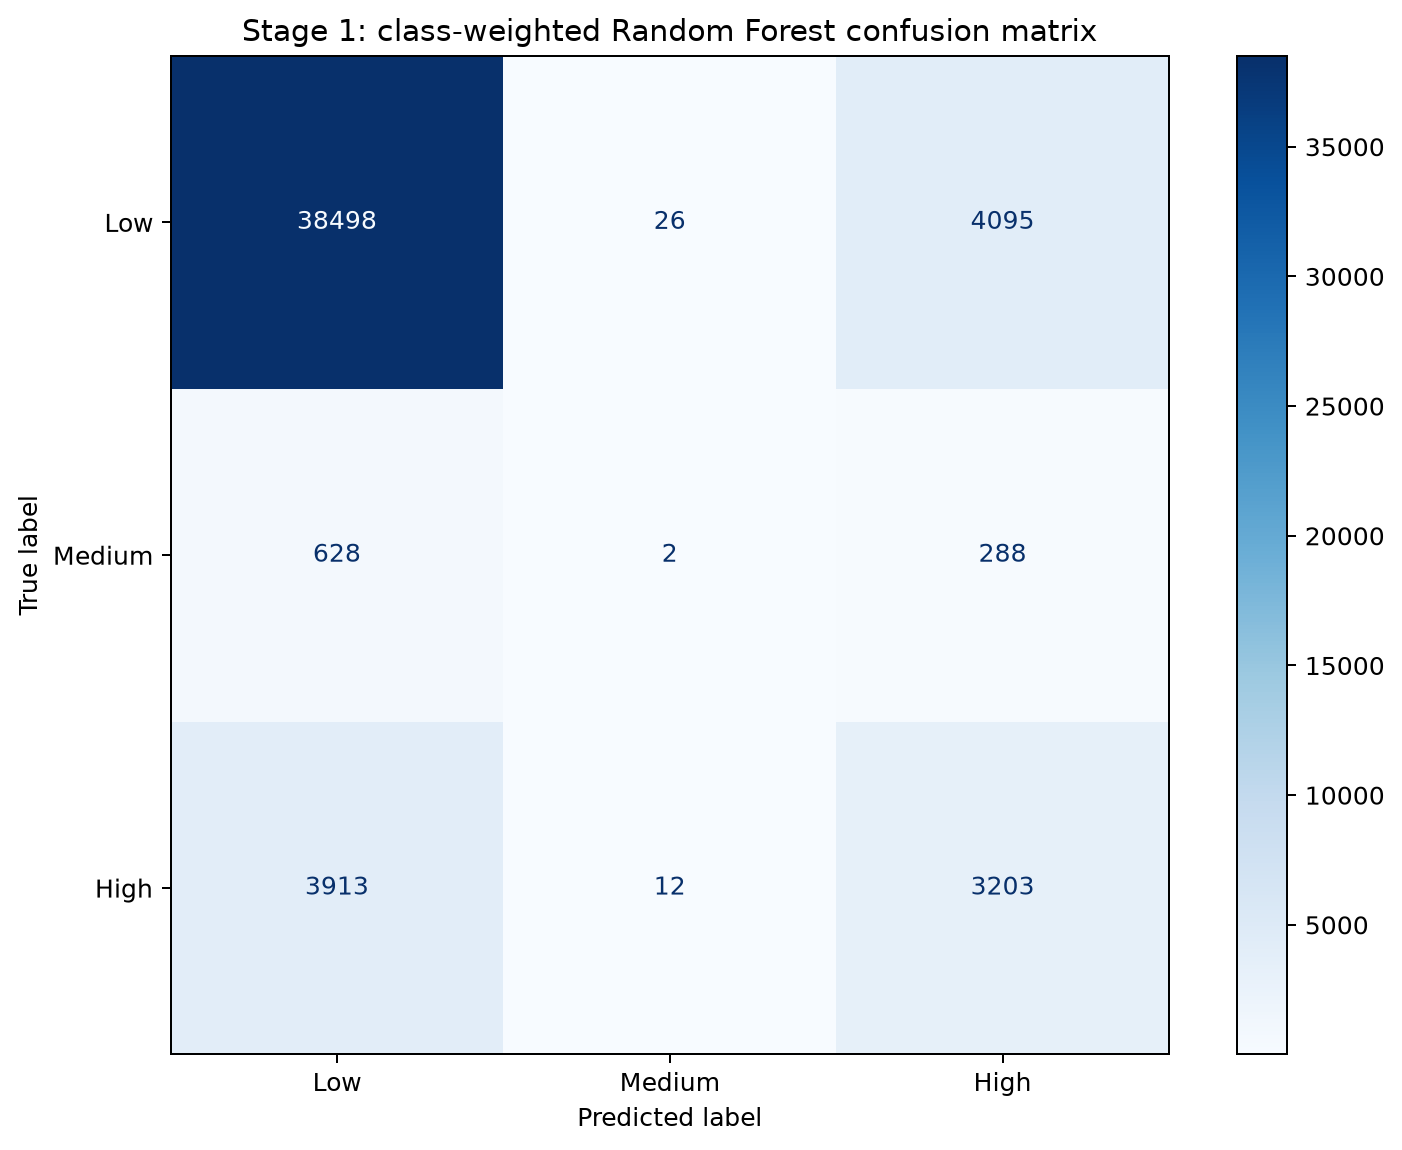
\includegraphics[width=0.82\linewidth]{artifacts_notebook/confusion_matrix.png}
\caption{Stage 1 confusion matrix for the held-out split. Only one of 926 Medium/prediabetes records is correctly classified.}
\label{fig:confusion}
\end{figure}

RQ1 is only partially supported. The model provides useful discrimination for Low and High labels but fails to identify Medium/prediabetes reliably.

\section{Experiment 2: Global and Patient-Level Explanation}

Global permutation importance uses 1,000 held-out records, three repeats, one worker, and seed 42. The leading features are general health (mean macro-F1 decrease 0.0458), BMI (0.0415), high blood pressure (0.0307), age (0.0259), and high cholesterol (0.0129). Negative lower-ranked values are not interpreted as protective medical effects.

\begin{figure}[t]
\centering
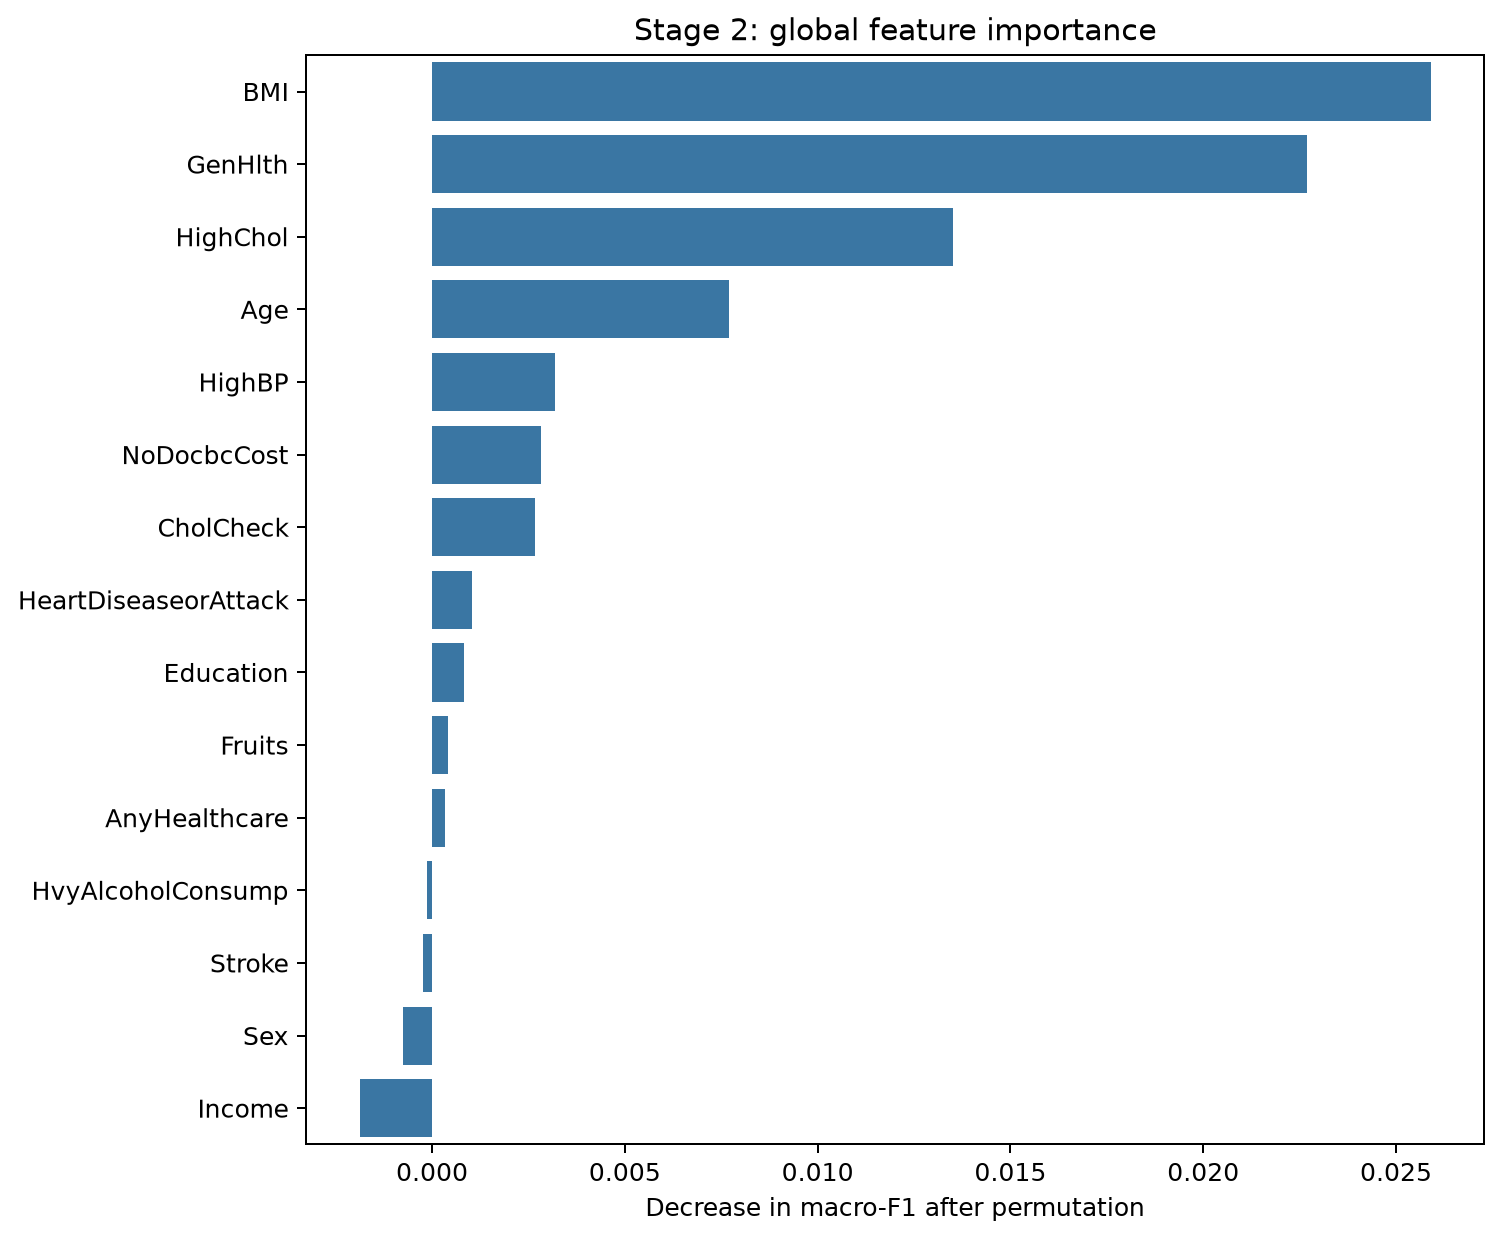
\includegraphics[width=0.75\linewidth]{artifacts_notebook/global_feature_importance.png}
\caption{Stage 2 global permutation importance measured by the decrease in held-out macro-F1 after shuffling.}
\label{fig:importance}
\end{figure}

The selected held-out record is dataset patient 104,917. Its recorded and predicted classes are High/diabetes, and the model assigns 56.69\% High/diabetes probability. The largest positive predicted-class SHAP contributions are BMI = 41 (+0.1200), GenHlth = 4 (+0.0874), and DiffWalk = 1 (+0.0616). The largest negative contributions are HighBP = 0 (-0.0778) and HighChol = 0 (-0.0422).

\begin{figure}[t]
\centering
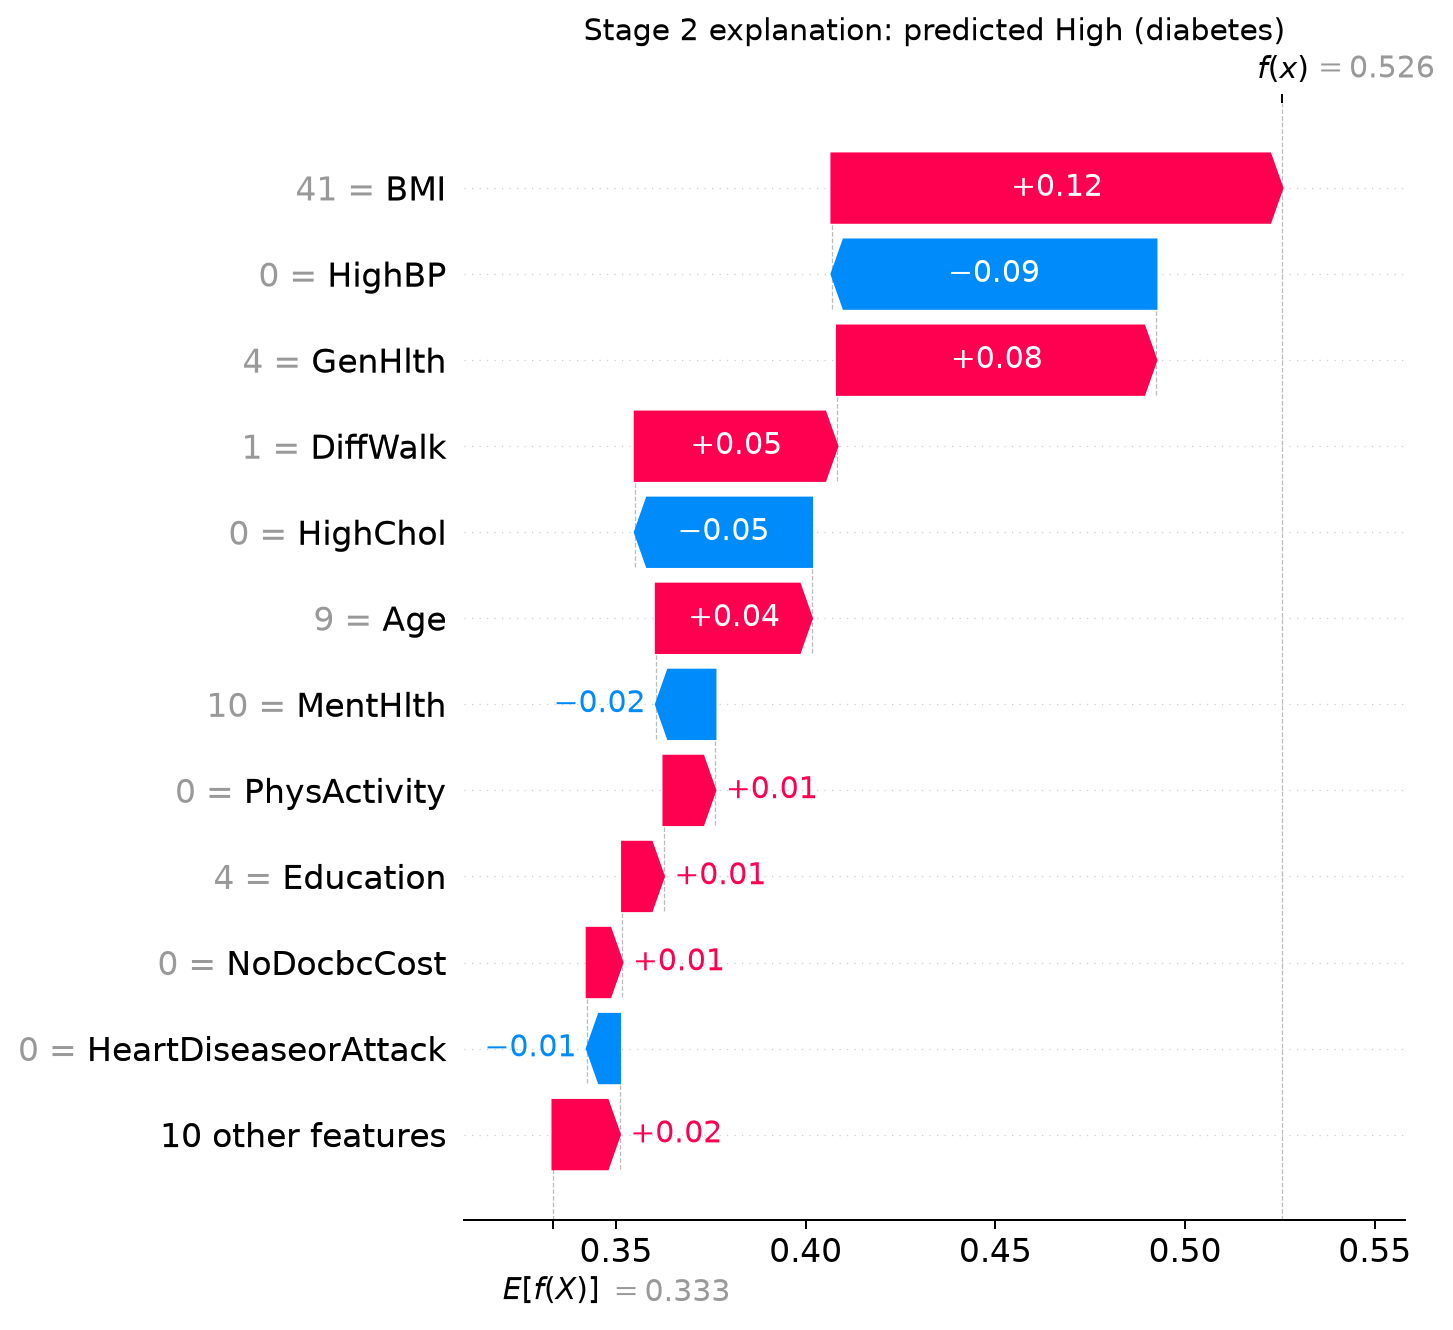
\includegraphics[width=0.8\linewidth]{artifacts_notebook/patient_shap_waterfall.png}
\caption{Exact predicted-class SHAP explanation for the held-out High/diabetes case. Contributions describe model support or opposition, not causation.}
\label{fig:shap}
\end{figure}

RQ2 is supported as a descriptive model-explanation question, not as evidence that a feature causes or prevents diabetes.

\section{Experiment 3: Manual What-If Digital Twin Scenario}

The manual scenario changes BMI from 41 to 36 and physical activity from 0 to 1 while holding the other 19 features fixed. The same model is then rerun without retraining. Table~\ref{tab:scenario} shows a 19.01 percentage-point reduction in High/diabetes probability.

\begin{table}[t]
\centering
\caption{Single-patient Stage 3 scenario. The change is a model re-prediction and not an intervention effect.}
\label{tab:scenario}
\begin{tabular}{lrrr}
\toprule
Quantity & Current & Scenario & Change \\
\midrule
BMI & 41.0 & 36.0 & -5.0 \\
Physical activity & 0 & 1 & +1 \\
High/diabetes probability & 56.69\% & 37.68\% & -19.01 points \\
SMPL beta 0 & 9.5 & 7.0 & -2.5 \\
\bottomrule
\end{tabular}
\end{table}

The 3D descriptor maps sex to the available SMPL model, BMI to the first shape coefficient, and High/diabetes probability to a display colour. These are visualization rules rather than physiological dynamics. RQ3 is therefore supported only as a transparent model what-if experiment.

\section{Experiment 4: Knowledge-Graph Evidence Integration}

The temporary graph includes six domains, all 21 observations, reusable definitions, decoded states, all 21 SHAP contributions, one prediction, three probabilities, model and evaluation metadata, and one Digital Twin representation. Patient-specific nodes are assembled in memory and are not written to Neo4j. SHAP links use explicit \texttt{SUPPORTS\_PREDICTION}, \texttt{OPPOSES\_PREDICTION}, or \texttt{NEUTRAL\_FOR\_PREDICTION} semantics. Earlier mechanistic nodes such as Insulin Resistance are removed.

Optional Ollama generation is restricted to selecting supplied feature and discussion-topic identifiers. The server validates the schema, signs, counts, uniqueness, and allow-listed topics before rendering deterministic prose. Invalid output is replaced by a deterministic evidence summary; raw local-model prose is not displayed.

The validation fixture produced 98 nodes and 135 edges, including 21 Observation nodes, 21 ShapContribution nodes, and three RiskProbability nodes. The fallback preserved the same patient evidence when Neo4j was unavailable. In the project environment, 22 focused implementation tests passed. RQ4 is supported for evidence integration and constrained guidance, not automatic clinical intervention generation.

\section{Discussion and Limitations}

The experiments have unequal evidential strength: Stage 1 is a 50,736-record held-out evaluation; Stage 2 uses a bounded importance sample and one local case; Stage 3 is one manually defined case study; and Stage 4 is primarily structural and safety testing. Their results must not be combined into a claim of clinical effectiveness.

The main strength is evidence continuity across one fixed 21-feature order. The main weakness is predictive validity, especially Medium/prediabetes recall. Further limitations include cross-sectional data, one split and model family, no uncertainty intervals, no external validation, a bounded permutation sample, a simplified 3D mapping, and no user or clinical evaluation. Docker Desktop was not running during the final report audit, so browser, live Neo4j, and Ollama behavior were not re-tested in that session.

\section{Conclusion}

We evaluated an explainable diabetes-risk Digital Twin as four separate but connected experiments. The Random Forest achieved moderate aggregate discrimination but failed on the Medium/prediabetes class. Permutation importance and local SHAP provided complementary descriptions of model behavior. A single manual scenario demonstrated consistent re-prediction and twin regeneration, while the knowledge graph preserved complete model evidence and constrained local-language-model output. The system should be presented as an evidence-oriented research prototype, not as a diagnostic tool, causal simulator, treatment recommender, or clinical decision-support system.

Future work should improve and repeatedly validate minority-class performance, report calibration and external generalization, expand explanation analysis to representative errors, and evaluate whether Stage 4 improves user understanding without increasing automation bias.

\begin{thebibliography}{9}
\bibitem{uci}
UCI Machine Learning Repository.
\newblock CDC Diabetes Health Indicators, Dataset 891.
\newblock \url{https://archive.ics.uci.edu/dataset/891/cdc+diabetes+health+indicators}.

\bibitem{breiman}
L. Breiman.
\newblock Random forests.
\newblock \emph{Machine Learning}, 45:5--32, 2001.
\newblock \url{https://doi.org/10.1023/A:1010933404324}.

\bibitem{lundberg}
S. M. Lundberg and S.-I. Lee.
\newblock A unified approach to interpreting model predictions.
\newblock \emph{Advances in Neural Information Processing Systems 30}, 2017.
\newblock \url{https://papers.nips.cc/paper_files/paper/2017/hash/8a20a8621978632d76c43dfd28b67767-Abstract.html}.

\bibitem{shen}
M.-D. Shen, S.-B. Chen, and X.-D. Ding.
\newblock The effectiveness of digital twins in promoting precision health across the entire population: a systematic review.
\newblock \emph{npj Digital Medicine}, 7:145, 2024.
\newblock \url{https://www.nature.com/articles/s41746-024-01146-0}.

\bibitem{connected}
F. Pianese et al.
\newblock CONNECTED: leveraging digital twins and personal knowledge graphs in healthcare digitalization.
\newblock 2023.
\newblock \url{https://pmc.ncbi.nlm.nih.gov/articles/PMC10733505/}.
\end{thebibliography}

\end{document}
